\documentclass[aps,prd,twocolumn,superscriptaddress,nofootinbib,showkeys]{revtex4-2}
\usepackage{amsmath,amssymb}
\usepackage{graphicx}
\usepackage{hyperref}
\hypersetup{pdftitle={Gravitation from Hilbert-Space Granularity: The Sphere, the String, and the Ring},pdfauthor={Andrew Korytko}}
\usepackage{booktabs}
\usepackage{array}
\usepackage[table]{xcolor}
\usepackage{orcidlink}
\usepackage{tikz}
\usetikzlibrary{arrows.meta}

\newcommand{\lc}{\ell_c}
\newcommand{\tc}{t_c}
\newcommand{\mc}{m_c}
\newcommand{\Ec}{E_c}
\newcommand{\ac}{a_c}
\newcommand{\RL}{R_\Lambda}
% A Software Heritage identifier, linked to its resolver, breakable after any character of its hash
\newcommand{\swhid}[1]{{\def\UrlBreaks{\do\:\do0\do1\do2\do3\do4\do5\do6\do7\do8\do9\do a\do b\do c\do d\do e\do f}\href{https://archive.softwareheritage.org/#1}{\nolinkurl{#1}}}}

% Display spacing: 6 pt above and below equations (REVTeX's default is 10 pt)
\makeatletter
\g@addto@macro\normalsize{\setlength{\abovedisplayskip}{6pt plus 2pt minus 2pt}\setlength{\belowdisplayskip}{6pt plus 2pt minus 2pt}\setlength{\abovedisplayshortskip}{2pt plus 1pt}\setlength{\belowdisplayshortskip}{4pt plus 1pt minus 1pt}}
% Section headings: 0.6 cm above and 0.35 cm below (REVTeX's default is 0.8 and 0.5 cm)
\def\section{\@startsection{section}{1}{\z@}{0.6cm \@plus1ex \@minus .2ex}{0.35cm}{\normalfont\small\bfseries}}
\def\subsection{\@startsection{subsection}{2}{\z@}{0.6cm \@plus1ex \@minus .2ex}{0.35cm}{\normalfont\small\bfseries}}
\makeatother
\begin{document}

\title{Gravitation from Hilbert-Space Granularity:\\ The Sphere, the String, and the Ring}

\author{Andrew Korytko\,\orcidlink{0009-0005-4569-2228}}
\email{andrew@alphalatitude.com}
\affiliation{AlphaLatitude Inc., P.O. Box 64341, Sunnyvale, California 94088, USA}

\date{September 23, 2026}

\begin{abstract}
For over a century, physics has sought a theory that unites general relativity and quantum mechanics. We argue that the answer has been staring us in the face: gravitation is what a granular quantum mechanics looks like at every scale. In Tim Palmer's Rational Quantum Mechanics, Hilbert space is granular, with a finite parameter $L$ that he attributes to gravity. We reverse the claim. $L$ comes first, one universal integer, and we start from two postulates: every qubit is a string of bits on a ring of cells, with no ring of more than $L$ cells, and any two cells not opposite lie on one ring of $L$ cells. The postulates give $L^2/4$ largest rings, and on the cosmological horizon each holds one bit of entropy. Jacobson's argument then gives Einstein's equations with $G = c^3\lc^2/(\pi\hbar\ln2)$, so the measured $G$ fixes the cell length $\lc$ at $\sqrt{\pi\ln2}$ Planck lengths. Newton's law, read as an equal share of energy per string, holds until a mass removes less entropy than a sphere's strings hold inside it, at the Newtonian acceleration $c^2/\pi\RL$; below it, galactic rotation curves flatten without dark matter, with $v^4 = a_MGM$ and $a_M = \pi c^2/12\RL = 1.4\times10^{-10}$~m\,s$^{-2}$, an upper bound, against $1.2$ observed. The largest ring fixes the cosmological constant, $G\Lambda = 12\pi c^3/(\hbar L^2\ln2)$. The cosmological and galactic scales, each with the measured $G$, give $L = 4.4\times10^{61}$ and $L \le 5.2\times10^{61}$, within 18\%. Only a quantum computer measures $L$ on its own, and that test will come within the decade. We predict a ceiling of $204$ qubits in a random state, the same for every technology. Every formula and number the paper derives is verified in Lean~4 from the postulates, thermodynamics, and elasticity.
\end{abstract}

\keywords{Rational quantum mechanics; discrete Hilbert space; emergent gravity; cosmological constant; galactic rotation curves; quantum computing}

\maketitle

\onecolumngrid
\begingroup
\refstepcounter{table}\label{tab:compare}
\vspace{-14pt}\noindent{\footnotesize TABLE~\thetable.\ ``Identical'': the derived formula equals the accepted one, so with $G$ and $\Lambda$ from experiment it gives the accepted value; nothing else is taken from it. Units: $\lc$ the cell, $n = r/\lc$, $\alpha = M/\mc$, $\ac = c^2/\lc$, $\Ec = \hbar c/\lc$, $\rho_c = \Ec/\lc^3$.}\par\vspace{2pt}
\begin{ruledtabular}
\footnotesize\setlength{\tabcolsep}{3pt}\renewcommand{\arraystretch}{0.95}
\begin{tabular}{>{\raggedright\arraybackslash}p{2.3cm}>{\raggedright\arraybackslash}p{5.2cm}>{\raggedright\arraybackslash}p{4.3cm}>{\raggedright\arraybackslash}p{5.2cm}}
Quantity & Derived from postulates, thermodynamics, and elasticity$^{\rm a}$ & Accepted & Status \\
\colrule
\arrayrulecolor{black!25}
Horizon entropy & one bit per largest ring, $(L^2/4)\ln2 = 3.3\times10^{122}$ & $A/4\ell_P^2 = 3.3\times10^{122}$ & Identical with $\lc$ from $G$: the quarter is Jacobson's for any count \\
\hline
Cell & $\lc = \sqrt{\pi\ln2\,\hbar G/c^3} = 2.39\times10^{-35}$~m & $\ell_P = \sqrt{\hbar G/c^3} = 1.62\times10^{-35}$~m & $\ell_P = \lc/\sqrt{\pi\ln2}$ derived; $G$ fixes the cell \\
\hline
Newton's constant & $4\pi c^3\RL^2/(\hbar L^2\ln2)$; a qubit ceiling of 204, $2^{204}\le L<2^{205}$, gives $4.8\times10^{-11}$ to $1.9\times10^{-10}$ & $6.674\times10^{-11}$~m$^3$\,kg$^{-1}$\,s$^{-2}$ & Inside the bracket by construction, $\log_2L = 204.8$ from $\Lambda$ and $G$; the ceiling makes it a factor-four test \\
\hline
Horizon temperature & $k_BT = \Ec/L = 3.0\times10^{-53}$~J & Gibbons--Hawking $\hbar c/2\pi\RL = 3.0\times10^{-53}$~J & Identical: $\hbar$ over the lap time \\
\hline
Newton's law & $a/\ac = \alpha/(\pi n^2\ln2)$; $5.93\times10^{-3}$~m\,s$^{-2}$ at 1~au & $GM/r^2 = 5.93\times10^{-3}$~m\,s$^{-2}$ & Identical: two Landauer energies per string of the sphere \\
\hline
Entropy a mass removes & $L\alpha$; Sun $5.9\times10^{99}$ & $2\pi Mc\RL/\hbar = 5.9\times10^{99}$ & Identical; the horizon shrinks by $\alpha/(\pi\ln2)$ cells \\
\hline
Galactic acceleration & $a_M = \pi c^2/12\RL = 1.42\times10^{-10}$~m\,s$^{-2}$, an upper bound & $a_0 = (1.20\pm0.24)\times10^{-10}$; $(1.19\pm0.10)\times10^{-10}$~m\,s$^{-2}$ & 85\% of the bound reached, $0.9\sigma$ and $2.3\sigma$; Verlinde's flat ball gives $0.90$ \\
\hline
Vacuum energy density & $3\pi^2\rho_c\ln2/2L^2 = 5.25\times10^{-10}$~J\,m$^{-3}$ & $\Lambda c^4/8\pi G = 5.25\times10^{-10}$; QFT estimate $10^{113}$ & Identical with $\RL$ from $\Lambda$; the 123 orders are $L^2$, a test once $L$ is measured \\
\hline
$G\Lambda$ & $12\pi c^3/(\hbar L^2\ln2) = 7.28\times10^{-63}$~m\,kg$^{-1}$\,s$^{-2}$ & $7.28\times10^{-63}$ & Identical; the content is $\propto1/L^2$ and $w = -1$ \\
\hline
Asymptotic Hubble rate & $2\pi/L\tc = 1.81\times10^{-18}$~s$^{-1}$ & $H_0\sqrt{\Omega_\Lambda} = 1.81\times10^{-18}$~s$^{-1}$ & Identical: $2\pi$ over the lap time of the horizon \\
\hline
Equation of state & $w = -1$ exactly & DESI DR2: evolving at $3.1\sigma$; Planck+BAO+SNe $-1.03\pm0.03$ & Tension; predicted not to survive \\
\hline
$L$ & $4.4\times10^{61}$ from $\Lambda$, $\le5.2\times10^{61}$ from galaxies, each with $G$ & --- & Agree to 18\%, which tests the galactic coefficient; the value from $\Lambda$ gives a ceiling of 204 \\
\hline
Qubit ceiling & 204 for every technology & none measured; 83-qubit circuits are consistent with $L\ge2^{83}$ & The test of the reversal; with $L$ measured, the rows with $L$ are tests \\
\arrayrulecolor{black}
\end{tabular}
\end{ruledtabular}
\vspace{3pt}\noindent{\footnotesize $^{\rm a}$Verified in Lean~4: the count from the postulates, each relation from them with thermodynamics and elasticity as named hypotheses, and each number from Appendix~\ref{app:numbers}. Of general relativity, only the Schwarzschild--de~Sitter solution is taken as already proven~\cite{kottler1918}.}\par
\endgroup
\vspace{8pt}
\twocolumngrid

\section{Introduction}

Rational Quantum Mechanics (RaQM)~\cite{palmer2020,palmer2026,palmer2026b,palmer2026c} leaves the Schr\"odinger equation untouched and instead restricts the bases in which a quantum state is defined: a qubit
\begin{equation}
|\psi\rangle = \cos\tfrac{\theta}{2}\,|1\rangle + e^{i\phi}\sin\tfrac{\theta}{2}\,|{-1}\rangle
\label{eq:qubit}
\end{equation}
with $\theta$ and $\phi$ the colatitude and azimuth of the state on the Bloch sphere, exists only in bases with
\begin{equation}
\cos^2\tfrac{\theta}{2} = \frac{m}{L},\qquad \frac{\phi}{2\pi} = \frac{n}{L},
\label{eq:raqm}
\end{equation}
with $m\in\{0,\dots,L\}$ and $n\in\{0,\dots,L-1\}$. The state is then a length-$L$ bit string whose fraction of $+1$ entries is $\cos^2(\theta/2)$ and whose cyclic shift by $n$ places is the phase~\cite{palmer2026}. Born's rule becomes a matter of counting. Bell's inequality is evaded because, by Niven's theorem~\cite{niven1956,jahnel2010}, the counterfactual measurement settings its derivation requires are not permitted bases~\cite{palmer2024,palmer2026b}. And because every probability is a frequency over $L$ bits, a random state of $N$ qubits needs $2^N \le L$, so there is a qubit capacity
\begin{equation}
N_{\max} = \lfloor\log_2 L\rfloor ,
\label{eq:nmax}
\end{equation}
beyond which quantum algorithms that spread their state across all of Hilbert space lose their exponential advantage~\cite{palmer2026}.

Palmer fixes $L$ from gravity. State reduction is a chaotic shift map that lowers $L$ by one each Planck time $t_P$ (in Palmer's ordering, $t_P = \sqrt{\hbar G/c^5}$), so the reduction time is $\tau^* = (L-1)t_P$. Equating this to the Di\'osi--Penrose collapse time $\hbar/E_G$~\cite{diosi1989,penrose1996} gives
\begin{equation}
L = \left\lceil\frac{E_P}{E_G}\right\rceil ,
\label{eq:palmerL}
\end{equation}
where $E_P = \hbar/t_P$ is the Planck energy, $E_G$ is the gravitational self-energy of the qubit's superposition, and $\lceil x\rceil$ is the smallest integer not less than $x$. Both $E_P$ and $E_G$ contain $G$. Gravity is the input and $L$ the output, and $L$ varies with the qubit, from $10^{64}$ for a quantum-dot electron to $10^{109}$ for a hyperfine ion-trap qubit~\cite{palmer2026}. Palmer closes by noting that his $N_{\max}$ lies near Davies' cosmological information bound~\cite{davies2007,lloyd2002} and that this is unlikely to be a coincidence.

We take that remark literally and reverse the causality. $L$ does not exist because of gravitation; gravitation exists because of $L$, one universal constant of nature. Table~\ref{tab:compare} shows what the reversal yields, with numbers on both sides; the sections below derive each row. We make the reversal concrete with two postulates that put Palmer's bit string on a ring of cells. A companion paper~\cite{korytko2026c} derives from them the probability of an outcome as a frequency, a unitary tick, and the Dirac equation along a line; nothing here depends on it.

Figure~\ref{fig:tree} shows the derivation, which runs one way. The postulates count the register, $L^2/4$ largest rings, and a largest ring, $L$ cells of length $\lc$, is a great circle of a sphere of radius $\RL = L\lc/2\pi$. A horizon is thermal and holds one bit on each of its rings, and a ring's share of that sphere is the area $4\lc^2/\pi$, so the entropy per unit area is $\pi k_B\ln2/4\lc^2$, whatever $L$ and $\RL$ are. From it and the thermodynamics of horizons follow Einstein's equations with $G = c^3\lc^2/(\pi\hbar\ln2)$, so the measured $G$ fixes the cell. In the weak field the equations give Newton's law, read as an equal share of energy per string. They leave the cosmological constant free, and Sec.~\ref{sec:cosmo} derives that the horizon of their solution without a mass is the sphere of the largest rings, which ties $\Lambda$ to $L$, so the measured $\Lambda$ gives us $L$'s reading from the cosmological scale. A second reading comes from the galactic scale. With an elastic response added, the count along a bit string gives the acceleration below which galactic rotation curves flatten, and from the measured $a_0$ we read off $L$ again. At each scale one structure of the register does the work: a sphere of strings, a string running to the horizon, and the closed ring. The two readings must agree, and the qubit ceiling, which the postulates alone give, must then find the same $L$ without $G$. Sections~\ref{sec:postulates} to \ref{sec:scales} follow the figure, from the postulates to the phenomena of each scale and what each scale pins. Section~\ref{sec:hold} asks whether $L$ holds, and Section~\ref{sec:predictions} lists what would falsify the picture.


\begin{figure*}[t]
\centering
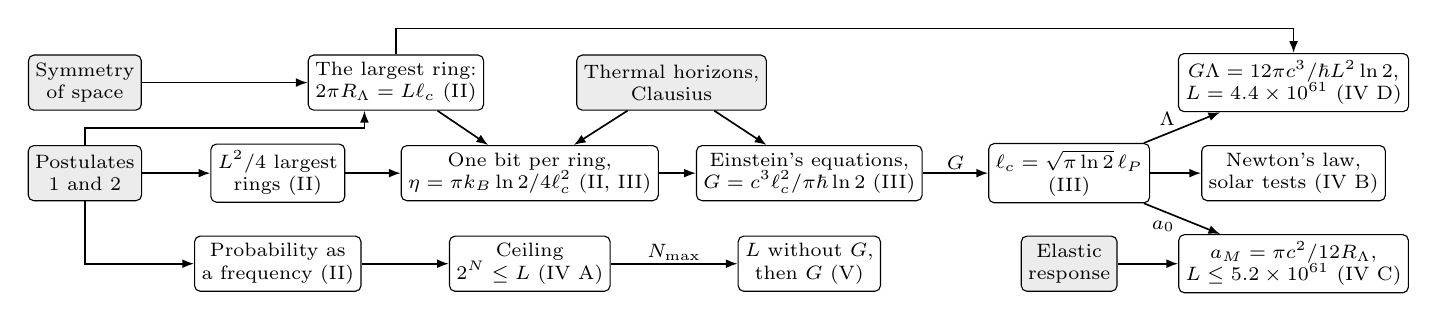
\begin{tikzpicture}[x=1cm,y=1cm,
  inp/.style={draw, fill=gray!15, rounded corners=2pt, align=center, font=\scriptsize, inner sep=2.5pt, minimum height=7mm},
  res/.style={draw, rounded corners=2pt, align=center, font=\scriptsize, inner sep=2.5pt, minimum height=7mm},
  arr/.style={-{Latex[length=1.5mm]}, semithick},
  lab/.style={font=\scriptsize, inner sep=1pt}]
\node[inp] (P)  at (0.80,0)   {Postulates\\1 and 2};
\node[res] (C)  at (3.25,0)   {$L^2/4$ largest\\rings (II)};
\node[res] (E)  at (6.45,0)   {One bit per ring,\\$\eta = \pi k_B\ln2/4\lc^2$ (II, III)};
\node[res] (EQ) at (10.0,0)   {Einstein's equations,\\$G = c^3\lc^2/\pi\hbar\ln2$ (III)};
\node[res] (LC) at (13.30,0)  {$\lc = \sqrt{\pi\ln2}\,\ell_P$\\(III)};
\node[res] (NW) at (16.15,0)  {Newton's law,\\solar tests (IV B)};
\node[res] (PL) at (4.75,1.15) {The largest ring:\\$2\pi\RL = L\lc$ (II)};
\node[inp] (TH) at (8.25,1.15) {Thermal horizons,\\Clausius};
\node[inp] (SY) at (0.80,1.15) {Symmetry\\of space};
\node[res] (GL) at (16.15,1.15) {$G\Lambda = 12\pi c^3/\hbar L^2\ln2$,\\$L = 4.4\times10^{61}$ (IV D)};
\node[res] (PR) at (3.25,-1.15) {Probability as\\a frequency (II)};
\node[res] (CE) at (6.45,-1.15) {Ceiling\\$2^N\le L$ (IV A)};
\node[res] (LQ) at (10.0,-1.15) {$L$ without $G$,\\then $G$ (V)};
\node[inp] (EL) at (13.30,-1.15) {Elastic\\response};
\node[res] (AM) at (16.15,-1.15) {$a_M = \pi c^2/12\RL$,\\$L\le5.2\times10^{61}$ (IV C)};
\draw[arr] (P) -- (C); \draw[arr] (C) -- (E);
\draw[arr] (SY) -- (PL);
\draw[arr] (P.north) -- ++(0,0.22) -| ([xshift=-4mm]PL.south);
\draw[arr] (PL) -- (E);
\draw[arr] (TH) -- (E); \draw[arr] (E) -- (EQ);
\draw[arr] (TH) -- (EQ);
\draw[arr] (EQ) -- node[lab, above]{$G$} (LC); \draw[arr] (LC) -- (NW);
\draw[arr] (LC) -- node[lab, above left, pos=0.45]{$\Lambda$} (GL);
\draw[arr] (PL.north) -- ++(0,0.33) -| (GL.north);
\draw[arr] (LC) -- node[lab, below left, pos=0.45]{$a_0$} (AM);
\draw[arr] (EL) -- (AM); \draw[arr] (P.south) |- (PR.west);
\draw[arr] (PR) -- (CE); \draw[arr] (CE) -- node[lab, above]{$N_{\max}$} (LQ);
\end{tikzpicture}
\caption{The derivation. Shaded boxes are inputs, labels on arrows are measured values, and no arrow runs back; the radius of the largest ring enters twice, in a ring's share of area and, once Sec.~\ref{sec:cosmo} shows it is the horizon's, in $\Lambda = 3/\RL^2$.}
\label{fig:tree}
\end{figure*}

\section{Postulates and Count}
\label{sec:postulates}

Two postulates define the register. A \emph{ring} is a closed line of translation in space; a \emph{cell} is a place on a ring; a \emph{tick} is the time light takes to cross a cell; a \emph{largest ring} is a ring of $L$ cells, the most a ring has (Postulate~1). A ring has no more than one bit per cell.

\textbf{Postulate 1 (the register).} \emph{Quantum mechanics is granular. Every qubit is a string of bits, one on each cell of a ring, each cell of length $\lc$, which light crosses in one tick. No ring has more than $L$ cells, with $L\in\mathbb{N}$. The bits are the possible outcomes of one measurement of the qubit, and the string's cyclic position on its ring is the qubit's phase. Any two qubits can be read jointly. The shift moves a bit to the next cell, a translation by one cell. A bit, and the measurement it answers, are carried from tick to tick. The global phase of a state is hidden: no law depends on it.}

\textbf{Postulate 2 (the rings).} \emph{Every cell has one opposite, the cell halfway around every largest ring through it. Any two cells not opposite lie on one largest ring, any two largest rings share a cell, and no ring holds every cell.}

We do not assume the length of a cell, $\lc$: Sec.~\ref{sec:count} derives $G$ in terms of it, and the measured $G$ then fixes it at $\sqrt{\pi\ln2}$ Planck lengths. The cell's tick, energy, mass, and acceleration are then $\tc = \lc/c$, $\Ec = \hbar c/\lc$, $\mc = \hbar/c\lc$, and $\ac = c^2/\lc$, and a mass $M$ is $\alpha = M/\mc$ cell masses. A ring of $L'$ cells has the lap time $L'\tc$. A massless mode with one wavelength around it completes one cycle per lap, so by Planck's relation it carries $h/L'\tc$, the least nonzero energy a massless mode on the ring can carry: the quantum of the ring.

Probabilities need no further postulate. A measurement returns the bit of one cell, and no law can pick which. A law that named the cell by its place would depend on where the cells are counted from, which is the global phase, and no law depends on it. A law that named it by its bit would need the arrangement of the bits, which is no part of the state: Postulate~1 gives a string's bits meaning as outcomes and its position as phase, and nothing else. Every cell is therefore read alike, so every probability is a frequency over the ring's bits: Eq.~(\ref{eq:raqm}) holds, with the ring's length for $L$, and Eq.~(\ref{eq:nmax}) holds as a ceiling (Sec.~\ref{sec:quantum}).

\textbf{The sphere.} A largest ring is $L$ cells of length $\lc$ on a closed line of translation, so it is a great circle of a sphere of radius
\begin{equation}
\RL = \frac{L\,\lc}{2\pi} ,
\label{eq:ident}
\end{equation}
the radius of the largest ring. By the symmetry of space a largest ring can run through a cell in any direction, so every great circle of that sphere is one. Any two largest rings share a cell (Postulate~2), which great circles of a sphere of three or more dimensions need not. So the sphere is a two-sphere, and space has three dimensions, as Ref.~\cite{korytko2026d} derives from postulates of its own. The count below is made on this sphere. Section~\ref{sec:cosmo} derives from Einstein's equations that it is the cosmological horizon of an observer at rest. Its radius is therefore measured, from $\Lambda$ (Sec.~\ref{sec:cosmo}) and from galactic rotation curves (Sec.~\ref{sec:galactic}), and with it $L$. The count uses only the area of the sphere, $A_{\rm hor} = 4\pi\RL^2 = L^2\lc^2/\pi$, and does not put the cells on it: it makes the largest rings the lines of a finite projective plane, in which, as for great circles, any two lines meet. Palmer's phase operator $\zeta$ is a cyclic permutation of the $L$-bit string, each application a rotation by exactly $2\pi/L$ about the polar axis~\cite{palmer2026}, so a full turn of phase takes $L$ steps. That those steps are the cells of a largest ring is not in his construction.

\textbf{The reversal.} We keep Palmer's picture of state reduction as a shift map at one step per tick, so that $\tau^* = L\tc$, but with $L$ universal. With $L$ a constant of nature the map cannot lower it; the reversal keeps only its clock, $L$ ticks. Then, by Eq.~(\ref{eq:ident}),
\begin{equation}
\tau^* = L\,\tc = \frac{2\pi\RL}{c} ,
\label{eq:clock}
\end{equation}
the time for one lap of a largest ring at the speed of light, $2\pi/H_\infty$ with $H_\infty = c/\RL$. The universal energy that replaces $E_G$ is then
\begin{equation}
\frac{\Ec}{L} = \frac{\hbar}{\tau^*} = \frac{\hbar c}{2\pi\RL} = k_B T_{\rm dS},
\label{eq:energy}
\end{equation}
the Gibbons--Hawking temperature of a horizon of radius $\RL$~\cite{gibbons1977}. Palmer's Eq.~(\ref{eq:palmerL}), read backwards, says that gravity's characteristic energy in the reduction process is the thermal energy of the cosmological horizon, and that every qubit shares it. Three consequences follow at once. First, $\tau^*\sim10^{11}$~yr, so an isolated qubit never completes reduction; Palmer makes the same observation. Second, $L$ no longer depends on the qubit, so $N_{\max}$ is the same for every technology, which is the sharpest experimental difference between the two causal orderings. Third, the reversal discards mass-dependent gravitational collapse, which Palmer's program takes to be gravity's role in quantum mechanics~\cite{palmer2016,hance2025}. In Palmer's ordering a heavy superposition has small $L$ and reduces in milliseconds; here every system shares the $10^{11}$-yr clock, so the definiteness of macroscopic bodies is not supplied by gravity and must come, as in standard quantum theory, from environmental decoherence. The reversed theory therefore predicts no mass-dependent collapse signal of Di\'osi--Penrose type, consistent with the null result of the underground search of Ref.~\cite{donadi2021}; Palmer's shift map is non-dissipative by construction and equally consistent with it, so the null result does not discriminate between the orderings, but $N_{\max}$ does.

\textbf{The count.} Postulate~2 fixes the number of cells and rings, and this count is the new input to gravity. An opposite lies halfway around a ring of $L$ cells, so $L$ is even. Every largest ring through a cell $P$ passes through its opposite $P'$, and two rings through $P$ share only $P$ and $P'$, since two cells not opposite fix one ring. So the rings through $P$ cut the remaining cells into disjoint sets of $L-2$. Any two largest rings share a cell (Postulate~2), and with it its opposite. Take a largest ring $A$ through $P$ and a cell $Q$ off it (Postulate~2). With $S$ a cell of $A$ other than $P$ and $P'$, the cells $Q$ and $S$ are not opposite, since the opposite of $S$ lies on $A$, so one largest ring $E$ passes through both. It misses $P$, since the one ring through $P$ and $S$ is $A$, which does not hold $Q$. Each ring through $P$ meets $E$ in one opposite pair, distinct rings in distinct pairs, and every pair of $E$ lies on a ring through $P$; $E$ has $L/2$ pairs, so $\rho = L/2$ rings pass through every cell. Every cell not opposite $P$ lies on one of them, so the register has
\begin{equation}
\begin{split}
C &= 2 + \rho(L-2) = \frac{L^2}{2} - L + 2 \ \text{cells},\\
R &= \frac{C\rho}{L} = \frac{L^2}{4} - \frac{L}{2} + 1 \ \text{rings},
\end{split}
\label{eq:counts}
\end{equation}
and $C = 2R$: one ring for every opposite pair of cells. With a cell and its opposite taken as a point and a largest ring as a line, the register is a finite projective plane of order $L/2 - 1$ (for $L\ge6$), with $R$ points and $R$ lines. That constrains $L$: every known plane has prime-power order, and orders $1$ or $2$ modulo $4$ that are not sums of two squares do not exist~\cite{bruck1949}. To leading order in $1/L$, a ring's share of the sphere's area is $A_{\rm hor}/R = 4\lc^2/\pi$.

\textbf{The entropy.} A horizon's entropy counts the strings that describe it, and a horizon holds as many as the register allows, one on each of its rings. Each contributes a doublet, which way its bits move (Postulate~1). The two directions of a mode of momentum $p$ carry the same energy, $|p|c$, so the horizon's thermal state (Sec.~\ref{sec:count}) weights them equally, and a doublet weighted equally holds one bit, $k_B\ln2$, the most a qubit can hold. So a horizon's entropy is one bit for each of its rings, and the sphere of the largest rings, the horizon of Sec.~\ref{sec:cosmo}, holds
\begin{equation}
\frac{S_{\rm hor}}{k_B} = R\ln2 = \frac{L^2}{4}\ln2
\label{eq:S}
\end{equation}
to leading order. It comes from the register's count, not from Bekenstein and Hawking; Sec.~\ref{sec:count} shows that, with the cell fixed by the measured $G$, it equals their quarter per Planck area.

\textbf{Counting in the bulk.} The count is exact on the sphere of the largest rings. A sphere of radius $r$ about a body has entropy proportional to its area, as every horizon does in Sec.~\ref{sec:count}, so it holds the fraction $(r/\RL)^2$ of the largest rings: its area in units of a ring's share. With $n = r/\lc$ the distance in cells,
\begin{equation}
N_s(r) = \frac{L^2}{4}\Big(\frac{r}{\RL}\Big)^2 = \pi^2 n^2
\label{eq:N}
\end{equation}
strings. These are shares of area, not places: at each distance from a body there are $L$ cells, two on each of its rings (Sec.~\ref{sec:galactic}). $L$ cancels between the count and the unit, so the counts on a sphere at solar radii do not involve $L$: they go as $n^2$, and $n^2 \ll L^2$. Areas, light cones, and the Raychaudhuri equation are written as in Jacobson's argument (Sec.~\ref{sec:count}); the register constructs no manifold, and what it adds is the count.

\section{Newton's Constant from the Count}
\label{sec:count}

Before testing the hypothesis at widely separated scales, we derive $G$ from the count of Sec.~\ref{sec:postulates} and the thermodynamics of horizons. Besides the symmetry of space (Sec.~\ref{sec:postulates}), two things are taken from outside the postulates, none of them a number. A horizon is thermal: its state is periodic in imaginary time, with the lap time of its ring as the period, and a state with imaginary-time period $\tau$ has temperature $k_BT = \hbar/\tau$, which is the Kubo--Martin--Schwinger condition~\cite{kubo1957,martin1959}. That the period is the lap time is the content of the Gibbons--Hawking and Unruh temperatures~\cite{gibbons1977,unruh1976}. The energy that crosses a horizon is heat, $\delta Q = T\,dS$, which is Jacobson's step~\cite{jacobson1995}, and with it goes his assumption that the entropy per unit area is the same on every horizon. The entropy comes from the register, Eq.~(\ref{eq:S}), which fixes that density. This is where we part from Jacobson's derivation, in which it is a free parameter that determines Newton's constant. Verlinde's entropic argument reaches Newton's law~\cite{verlinde2011}; we do not use it, since it treats gravity as a force driven by the entropy of a screen, the step that is contested~\cite{visser2011,kobakhidze2011}, whereas Jacobson's argument involves no force. The elastic response of his later work~\cite{verlinde2017} is a different argument, and Sec.~\ref{sec:galactic} uses it.

\subsection{The temperature of a horizon in cells}
A horizon's ring of $L_h$ cells has the lap time $L_h\tc$, and by the thermal assumption its temperature is
\begin{equation}
k_B T = \frac{\hbar}{L_h\tc} = \frac{\Ec}{L_h} .
\label{eq:T}
\end{equation}
For a horizon of largest rings, $L_h = L$, the lap time is $2\pi\RL/c$, and Eq.~(\ref{eq:T}) is Eq.~(\ref{eq:energy}). An observer accelerating at $a$ has a horizon $c^2/a$ behind him, whose imaginary-time period is $2\pi c/a$, the lap time of a ring of $L_a = 2\pi c^2/a\lc$ cells; Eq.~(\ref{eq:T}) then gives $k_BT_a = \hbar a/2\pi c$, Unruh's temperature. The register supplies the quantum of every ring, $h$ over its lap time, and the temperature is that quantum over $2\pi$. Through every point of spacetime, in every null direction, passes the horizon of such an observer, a local Rindler horizon.

\subsection{Clausius relation}
On every local Rindler horizon the entropy is one bit for each of its rings, so Jacobson's balance of heat and entropy reads
\begin{equation}
\delta Q = T_a\,dS = k_BT_a\ln2\,dR = \frac{\hbar a\ln2}{2\pi c}\,dR :
\label{eq:clausius}
\end{equation}
each ring a horizon gains takes in $k_BT_a\ln2$, its temperature times one bit of entropy, which is Landauer's energy of a bit~\cite{landauer1961}. Energy crossing a horizon therefore adds rings, $2\pi c/(\hbar a\ln2)$ of them per unit of energy, and with a ring's share of area $4\lc^2/\pi$ it adds area $dA = [8\lc^2 c/(\hbar a\ln2)]\,\delta Q$. The Raychaudhuri equation gives the change of area in terms of the Ricci tensor, and the balance can hold in every direction at every point only if
\begin{equation}
R_{\mu\nu} - \tfrac12 R\,g_{\mu\nu} + \Lambda g_{\mu\nu} = \frac{2\pi k_B}{\hbar c\,\eta}\,T_{\mu\nu},
\label{eq:einstein}
\end{equation}
with $\eta$ the entropy per unit area and $\Lambda$ an integration constant that the argument leaves free. A stress tensor proportional to the metric has no flux through a null surface, so it never enters Eq.~(\ref{eq:clausius})~\cite{jacobson1995,korytko2026b}. This is Einstein's equation, and comparing its coefficient with $8\pi G/c^4$ gives $G = c^3k_B/4\hbar\eta$. Nothing in this is a force: Eq.~(\ref{eq:einstein}) is a condition on the geometry, that the count of every local horizon stays in balance with the heat that crosses it, and matter then moves on the geodesics of the geometry that satisfies it.

\subsection{The cell from Newton's constant}
By Eqs.~(\ref{eq:counts}) and (\ref{eq:S}) the entropy per unit area of the horizon is, to leading order in $1/L$, $\eta = k_B R\ln2/A_{\rm hor} = k_B(L^2/4)\ln2/(L^2\lc^2/\pi)$, so
\begin{equation}
\eta = \frac{\pi k_B\ln2}{4\lc^2}, \qquad
G = \frac{c^3\lc^2}{\pi\hbar\ln2} = \frac{4\pi c^3\RL^2}{\hbar L^2\ln2} .
\label{eq:G}
\end{equation}
This is the result of the section. The $\pi$ comes from a ring's share of area, $4\lc^2/\pi$, and the $\ln2$ from the bit; Jacobson's $4$, from the $8\pi$ of the field equations and the $2\pi$ of the thermal period, cancels the $4$ of that share. Newton's constant is measured, so Eq.~(\ref{eq:G}) fixes the cell,
\begin{equation}
\lc = \sqrt{\frac{\pi\ln2\,\hbar G}{c^3}} = \sqrt{\pi\ln2}\,\ell_P = 2.39\times10^{-35}~{\rm m},
\label{eq:cell}
\end{equation}
with $\ell_P \equiv \sqrt{\hbar G/c^3} = \lc/\sqrt{\pi\ln2}$,
so the Planck length is a derived quantity, the cell over $\sqrt{\pi\ln2}$. With it the horizon's entropy, Eq.~(\ref{eq:S}), is $S_{\rm hor}/k_B = (L^2/4)\ln2 = \pi^2\RL^2\ln2/\lc^2 = \pi\RL^2/\ell_P^2 = A_{\rm hor}/4\ell_P^2$: Bekenstein and Hawking's quarter per Planck area~\cite{bekenstein1973} is the register's one bit per ring, a ring's share of the horizon being $4\ell_P^2\ln2$. The quarter itself follows from Jacobson's coefficient and the measured $G$ for any count; the count fixes the cell. Newton's law, $a = GM/r^2$, is the weak-field limit of Eq.~(\ref{eq:einstein}). Its content for a static sphere is Padmanabhan's equipartition~\cite{padmanabhan2010}, which holds in every static solution of Eq.~(\ref{eq:einstein}). The Komar energy inside a sphere on which the acceleration is $a$, the energy that gravitates, is twice its entropy times the temperature, $Mc^2 = 2T_aS$~\cite{komar1959}, two Landauer energies $k_BT_a\ln2$ for each of its strings,
\begin{equation}
\begin{split}
Mc^2 &= 2N_s(r)\,k_BT_a\ln2 = \pi n^2\ln2\,\frac{\hbar a}{c}\\
&\Longrightarrow\quad \frac{a}{\ac} = \frac{\alpha}{\pi n^2\ln2} ,
\end{split}
\label{eq:newton}
\end{equation}
with $\alpha = M/\mc$ and $n = r/\lc$. So Newton's law reads: the body's energy is shared equally by the strings of any sphere around it; the share per string is set by the temperature of the horizon that an observer held on the sphere sees; and the share falls as $1/r^2$, since the number of strings grows as $r^2$. A test body $n$ cells from a mass of $\alpha$ cell masses accelerates at $\alpha/(\pi n^2\ln2)$ in units of $\ac$. Two remarks follow. First, a continuum does not gravitate: without cells the entropy per area of a horizon diverges with the cutoff, $\eta\to\infty$, and $G\to0$, since no finite energy changes the area of a horizon that holds infinitely many strings per unit of area. Finite cells gravitate because each ring is worth $4\lc^2/\pi$ of area, and Eq.~(\ref{eq:clausius}) is the exchange rate. Second, Eq.~(\ref{eq:G}) scales as $1/L^2$: with $L$ a constant of nature, $G$ is constant exactly when the horizon radius is; this singles out the de Sitter horizon (Sec.~\ref{sec:cosmo}) and makes the constancy of $G$ and of $\Lambda$ one statement (Sec.~\ref{sec:predictions}). The numerical value of $G$ follows from a measurement of $L$ that does not use $G$, and a quantum computer's qubit ceiling is that measurement (Sec.~\ref{sec:hold}).

\section{Gravitational Phenomena Scale by Scale}
\label{sec:scales}

On each scale one structure of the register does the work, and we record what each scale pins. At the solar scale it is the sphere of Eq.~(\ref{eq:N}); at the galactic scale the string, a largest ring whose cells run from the sphere out to the horizon, $L/4$ cells from the body; at the cosmological scale the closed ring.

\subsection{Quantum scale: qubits and quantum computers}\label{sec:quantum}

Here $L$ acts directly through Eq.~(\ref{eq:nmax}), and the joint reading of Postulate~1 shows which states it limits. When a state is read jointly, the cells on which the earlier qubits show an outcome that leaves a later qubit in one state form a \emph{block} of the later string, and the string's fraction of 1s and position in that block give that state. Outcomes that leave the qubit in the same state therefore share a block, and the probability of a joint outcome is the product, string by string, of the frequencies of its bits on its blocks. A block whose fraction lies strictly between 0 and 1 needs at least two cells, one reading 1 and one reading 0. In a random state, each of the $2^{N-1}$ joint outcomes of the first $N-1$ qubits leaves the last in a different state, with probability strictly between 0 and 1. Its string then needs $2^{N-1}$ blocks of at least two cells, so $2^N$ is at most its length, and $2^N\le L$. A product state needs one block per string, and a state of the Greenberger--Horne--Zeilinger type only blocks of fraction 0 or 1, which need one cell each, so neither tests the bound at any $N$. Random-circuit sampling does. The $53$-, $70$- and $83$-qubit experiments of Refs.~\cite{arute2019,morvan2024,gao2025} are consistent with $2^{83}\le L$, though at cross-entropy fidelities below 1\% they do not establish it, and 83 is in any case far below $\log_2L = 204.8$, so this scale does not yet pin $L$. Physical qubit counts are much larger: a single tweezer array holds $6{,}100$ atoms~\cite{manetsch2025}. But a count of physical qubits is not a count of qubits in a random state, and the bound says nothing about it. Nor do the local observables measured after a many-body quench test it: they do not tell a random state from a mixed one, and only the return under the reversed evolution does. Logical qubits count as physical ones do: a logical qubit is a qubit, so Postulate~1 gives it a string, and the $48$ demonstrated on $280$ atoms~\cite{bluvstein2024} lie far below the ceiling. On the timescale Palmer gives for factoring tests~\cite{palmer2026,gidney2025}, this scale will measure $L$ directly. The test is a random circuit on $N$ fault-tolerant logical qubits, deep enough to produce a random state, followed by its inverse. In quantum mechanics the state returns to the initial one with the gate fidelity; here it does not once $N$ exceeds $\log_2L$, because the intermediate state needs more blocks than its last string has room for. By how much it fails to return is not derived here, only the $N$ at which it starts. Error correction does not lift the ceiling, which is set by room and not by errors. The reversed theory's prediction on this scale is $N_{\max} = 204$, the same for every technology (Sec.~\ref{sec:hold}).

State reduction on this scale runs on the universal clock (\ref{eq:clock}) and never completes; nothing observable changes for laboratory qubits, exactly as in RaQM.

\subsection{Terrestrial and solar scales: the sphere}

Section~\ref{sec:count} gave Einstein's equations with $G = c^3\lc^2/(\pi\hbar\ln2)$, Eq.~(\ref{eq:G}), and Newton's law as their weak-field limit, Eq.~(\ref{eq:newton}). Gravitational redshift~\cite{pound1960}, the perihelion advance of Mercury, light deflection, and gravitational-wave propagation then follow as they do in general relativity. Mercury's anomalous advance $6\pi GM_\odot/(p\,c^2)$, with $p = a_{\rm orb}(1-e^2)$ the semi-latus rectum of the orbit, is $42.98''$ per century and the deflection of starlight at the solar limb $4GM_\odot/(c^2R_\odot)$ is $1.75''$, both as observed. At the Earth's orbit, $\alpha = 1.35\times10^{38}$ and $n = 6.27\times10^{45}$ in Eq.~(\ref{eq:newton}) give $5.93\times10^{-3}$~m\,s$^{-2}$. They depend on $L$ and $\RL$ only through $G$, i.e., only through the cell $\lc = 2\pi\RL/L$.

This scale therefore pins $\lc$, the combination $2\pi\RL/L$, and not $L$ on its own. The count of a sphere is $n^2$, with $L$ cancelled against the unit, Eq.~(\ref{eq:N}); and the horizon of an observer held at solar radii is his own, $L_a\ll L$, since $a\gg c^2/\RL$ there. This is as it should be, since solar-system gravity is described by general relativity to exquisite precision, and a theory in which $L$ showed up there separately from $\RL$ would be wrong. The situation is the gravitational analogue of Palmer's observation that RaQM and QM are indistinguishable for small numbers of qubits: the granularity shows itself only at the extremes, at large $N$ in the quantum case and at small acceleration in the gravitational case. To forestall a natural misreading: the direct kinematic effect of a $2\pi/L$ phase grid on an orbit is $\sim10^{-61}$~rad per revolution, fifty-four orders of magnitude below Mercury's $5\times10^{-7}$~rad; angular discreteness does nothing to orbits. The horizon could enter solar-system dynamics by two routes. The push of Sec.~\ref{sec:cosmo} reaches the planets, but with only $5\times10^{-25}$~m\,s$^{-2}$ at the Earth's orbit. For an isolated Sun the elastic response of Sec.~\ref{sec:galactic} stops short of them: a sphere about the Sun is saturated, and Newton's law holds exactly, out to the crossing of Eq.~(\ref{eq:criterion}), where $GM_\odot/r^2 = c^2/\pi\RL$, $5900$~au from the Sun. The Sun is not isolated, though. In modified-Poisson versions of MOND the Galaxy's field adds a quadrupole to the Sun's, which Cassini's ranging bounds at $Q_2 = (3\pm3)\times10^{-27}$~s$^{-2}$, excluding the standard transitions~\cite{hees2014} and in tension with the radial acceleration relation~\cite{desmond2024}. The counts above are for an isolated mass and do not say whether the register has such an effect; the bound is a test it must pass.

\subsection{Galactic scale: the string}\label{sec:galactic}

At the scales above, $L$ and $\RL$ entered gravity only through their ratio, and two facts of the register played no part. The strings counted have $L$ bits, one on each cell of a largest ring, which reaches the horizon: the strings counted on a sphere are not confined to it. And no ring has more than $L$ cells, so no horizon is colder than $\Ec/L$. The floor is on the temperature, not on the acceleration: in de Sitter space an observer held at acceleration $a$ sees the two horizons combined in quadrature, $k_BT = (\hbar/2\pi c)\sqrt{a^2 + a_\Lambda^2}$ with $a_\Lambda = c^2/\RL$~\cite{deser1997}, never below $\Ec/L$, whatever $a$ is. Both facts enter at accelerations of order the horizon's surface gravity, $c^2/\RL = cH_\infty = 5.4\times10^{-10}$~m\,s$^{-2}$. That the scale at which rotation curves flatten is the horizon's acceleration, up to a coefficient, is not ours: Milgrom reached it from the Unruh temperature of de Sitter space~\cite{milgrom1999}, and Verlinde from its entanglement entropy~\cite{verlinde2017}. Ours is the count that fixes where $L$ enters, and the coefficient, which we now derive by following Verlinde's elastic argument with the register's counts in place of his entropy assignments.

\textit{A mass draws the horizon in.} Einstein's equations were derived in Sec.~\ref{sec:count}. Their solution for a mass $M$ inside the cosmological horizon is Schwarzschild--de Sitter~\cite{kottler1918}, whose outer horizon lies at $\RL - GM/c^2$ to first order in $M$. By Eq.~(\ref{eq:cell}), $GM/c^2 = \lc\alpha/(\pi\ln2)$: the mass draws the horizon in by $\alpha/(\pi\ln2)$ cells. Its circumference loses $2\alpha/\ln2$ cells, and since the entropy is $(\ln2)/4$ times the square of the circumference in cells, Eq.~(\ref{eq:S}), the loss is $(L/2)\cdot(2\alpha/\ln2)\cdot\ln2$,
\begin{equation}
S_M = L\alpha = \frac{Mc^2}{k_BT_{\rm dS}} = \frac{2\pi Mc\RL}{\hbar} ,
\label{eq:SM}
\end{equation}
which is Verlinde's result, Eq.~(25) of Ref.~\cite{verlinde2017}, in cells. The entropy a mass takes from the horizon is its mass in cell masses times the length of the ring in cells, or its energy over the horizon's temperature, and it does not depend on the cell's size. For the Sun $L\alpha = 5.9\times10^{99}$; for a galaxy of $10^{11}M_\odot$, $5.9\times10^{110}$. Within a sphere of radius $r\ll\RL$ the mass removes entropy the same way. A sphere's area grows with geodesic distance at $8\pi$ times its radius less $8\pi GM/c^2$, so out to $r$, far outside the body, it falls short by $8\pi GMr/c^2$. At a ring's share $4\lc^2/\pi$ that is $2\pi n\alpha/\ln2$ rings, one bit each, so the mass removes $S_M(r) = 2\pi n\alpha = 2\pi Mcr/\hbar$. At $r = \RL$ this is Eq.~(\ref{eq:SM}), and it agrees with Verlinde's Eq.~(28).

\textit{Where the strings hold their entropy.} The sphere at $r$ has $N_s(r) = \pi^2n^2$ strings, Eq.~(\ref{eq:N}), the horizon's $L^2/4$ scaled by the ratio of areas, but its strings are not confined to it: each lies on a largest ring through a cell of the sphere, and the ring runs on to the horizon. Postulate~2 gives every cell not opposite the body a distance from it, the number of steps from cell to cell, the shorter way round, along the one largest ring through both. The body's opposite lies $L/2$ out along all of the body's $L/2$ rings, and at each distance in between there are $L$ cells, two on each ring. The horizon of a body at rest lies $L/4$ cells out, since the de Sitter solution of Eq.~(\ref{eq:einstein}) puts it at the proper distance $\pi\RL/2 = L\lc/4$, a quarter of a largest ring. Along a ring the distance is proper distance; it equals the areal radius of Eq.~(\ref{eq:N}) for $r\ll\RL$, the only case used below, and at the horizon the two are $L/4$ and $L/2\pi$. The two cells of an opposite pair lie at the distances $d$ and $L/2 - d$, one on each side of the horizon or both on it, and every largest ring is made of $L/2$ such pairs, since it passes through the opposite of each of its cells. So every string has half its cells, $L/2$ of them, inside the horizon, counting a cell on it as half. Its entropy, one bit, is which way it moves. The body's observer never sees beyond his horizon (Sec.~\ref{sec:cosmo}), so his description of a string is its half inside; every bit carries that direction alike (Postulate~1), so that half holds the whole bit, spread evenly over its $L/2$ cells, since no law picks a cell (Sec.~\ref{sec:postulates}).

The largest rings through a cell $P$ of the sphere, apart from the one through the body, hold between them every cell off that ring exactly once. Such a cell is not opposite $P$, so one largest ring passes through both, and it is not the ring through the body. Besides $P$ and its opposite, which lie on all of them, these rings hold $L-2$ cells at each distance from $1$ to $L/2-1$, and the ring through the body holds two. So the rings through $P$ spread their cells inside the horizon evenly over the distances up to $L/4$, and $n$ of every $L/4$ lie inside the sphere. To leading order in $1/n$, the entropy the sphere's strings hold inside it is therefore the fraction $n/(L/4) = 4n/L$ of their $N_s(r)$ bits,
\begin{equation}
S_{\rm in}(r) = \frac{4n}{L}\,N_s(r)\ln2 = \frac{4\pi^2 n^3}{L}\ln2 ,
\label{eq:volume}
\end{equation}
a volume law. Verlinde postulates a volume law for the entanglement entropy of de Sitter space, the horizon entropy divided evenly over the bulk, and normalizes it on a flat ball of radius $\RL$, which gives the fraction $2\pi n/L$. His Eq.~(81) says that each cell of the sphere contributes the fraction given by the ratio of the proper distances from the center to that cell and to the horizon. In the register that ratio is a count, $n$ over $L/4$. The horizon is at $\pi\RL/2$ along a ring, not at $\RL$, and that is the whole difference between our $\pi/12$ and his $1/6$. The volume law itself, which Verlinde postulates, follows here from the count. While the mass removes more entropy within the sphere than its strings hold there, $S_M(r) > S_{\rm in}(r)$, the sphere is saturated: what fixes the share is the two-dimensional count of Eq.~(\ref{eq:N}), and Newton's law holds. The crossing is where the two are equal,
\begin{equation}
S_M(r) = S_{\rm in}(r): \quad N_s = \frac{\pi L\alpha}{2\ln2}, \quad g_N = \frac{c^2}{\pi\RL} ,
\label{eq:criterion}
\end{equation}
so rotation curves depart from Newton's law at an acceleration of order the horizon's, with the coefficient fixed by the count.

\textit{The elastic response.} Below the crossing the entropy inside the sphere exceeds what the mass removes, and the remainder responds as an incompressible elastic medium. The removed entropy occupies the volume $V_M = S_M(r)\,V_0$, with $V_0 = V(r)/S_{\rm in}(r) = L\lc^3/(3\pi\ln2)$ the volume per unit of entropy from Eq.~(\ref{eq:volume}). The strain $\varepsilon$ outside the removed region obeys $\int_0^r \varepsilon^2 A\,dr' \le V_M(r)$, with equality under Verlinde's assumption on the principal strain, his Eqs.~(44)--(46) and (88), and the strain gives the apparent surface mass density, $\Sigma_D = (a_\Lambda/8\pi G)\,\varepsilon$ with $a_\Lambda = c^2/\RL$, his Eq.~(43). The energy of a strain is quadratic in it, which is why the apparent mass goes as the square root of the removed entropy rather than in proportion to it. With equality, differentiating at fixed $M$ gives $\varepsilon^2 = (1/A)\,dV_M/dr$, and with Gauss's law $\Sigma = g/4\pi G$,
\begin{equation}
g_D^2 = a_M\,g_N, \quad a_M = \frac{\pi}{12}\,\frac{c^2}{\RL} = 1.42\times10^{-10}~{\rm m\,s^{-2}} ,
\label{eq:aM}
\end{equation}
which is $(\pi^2/6)\,c^2/L\lc$. Without equality, Eq.~(\ref{eq:aM}) is an upper bound on the deep regime. There the apparent mass $M_D$ grows as $r$, so $\varepsilon^2A$, which goes as $(M_D/r)^2$, tends to a constant. The mean of $\varepsilon^2A$ out to $r$, which the inequality keeps below $V_M/r = dV_M/dr$, tends to the same constant, and so the constant is at most $dV_M/dr$. The apparent dark mass is $M_D = M\,n\sqrt{\pi^3\ln2/6L\alpha}$: it grows by a fixed amount per cell of distance, as the part of a string inside the sphere does: the string is the structure of this scale. Verlinde's own normalization gives $a_M = c^2/6\RL = 0.90\times10^{-10}$~m\,s$^{-2}$, his Eq.~(102); the register's coefficient is $\pi/2$ larger. The total field is $g = g_N + g_D$, and in the deep regime, where $g_D\gg g_N$,
\begin{equation}
g = \sqrt{a_M\,g_N},\qquad v_c^4 = a_M\,G\,M ,
\label{eq:btfr}
\end{equation}
flat rotation curves and the baryonic Tully--Fisher relation, with $M$ the baryonic mass alone. This is Milgrom's phenomenology~\cite{milgrom1983}, confirmed as a tight empirical law across galaxy types by the radial acceleration relation~\cite{mcgaugh2016}, with one $a_0$ for galaxies whose stellar masses span five orders of magnitude. The measured scale is $a_0 = (1.20\pm0.02\pm0.24)\times10^{-10}$~m\,s$^{-2}$~\cite{mcgaugh2016}, and $(1.19\pm0.04\pm0.09)\times10^{-10}$ when each galaxy's distance, inclination and mass-to-light ratios are fitted along with it~\cite{desmond2023}. Equation~(\ref{eq:aM}) lies $0.9\sigma$ above the first and $2.3\sigma$ above the second: observation reaches 85\% of the bound. With Verlinde's normalization the observed $a_0$ would exceed the bound. For attribution, the coefficients in units of $cH_\infty$ are: $1$, Milgrom's vacuum scale~\cite{milgrom1999}; $2$, the de Sitter temperature in an equipartition~\cite{hominicng2010}; $1/6 = 0.17$, Verlinde~\cite{verlinde2017}; $0.13$ after the correction of Refs.~\cite{yoon2025,yoon2023}; $\pi/12 = 0.26$, this paper; against $0.22$ observed. The Tully--Fisher speed of a $10^{11}M_\odot$ galaxy is $208$~km\,s$^{-1}$ by Eq.~(\ref{eq:btfr}), against $200$ observed. Verlinde's specific interpolation between the Newtonian and deep regimes shows tension with the radial acceleration relation in the transition region~\cite{lelli2017}; what pins $L$ here is the deep-regime scaling (\ref{eq:btfr}), which survives that test, and the transition function remains open.

\textit{Why the temperature cannot lead.} The floor $\Ec/L$ could be taken as the mechanism instead of the bits. If gravity followed the excess of the combined temperature over the floor, as Milgrom proposed~\cite{milgrom1999}, Eq.~(\ref{eq:newton}) would give $a = \sqrt{g_N^2 + 2a_\Lambda g_N}$. That has the right deep form, with $a_M = 2c^2/\RL$, nine times the observed value, and a transition 38\% above Newton's law at $g_N = 10a_0$, where the observed relation is 4\% above. The floor marks the scale; the law is in the strings.

To be explicit: in this framework there is no dark-matter halo, nor the smearing of energy-momentum over neighboring space-times by which Invariant Set Theory reaches the same phenomena with $\Lambda = 0$~\cite{palmer2016,hance2025}. Galactic rotation is set by the baryons, $G$, and the horizon radius, which $\Lambda$ fixes. The known difficulties of any such account, galaxy clusters~\cite{clowe2006} and the acoustic peaks of the microwave background~\cite{planck2018}, are not addressed here and remain open.

This scale pins $L$. The deep-regime law is observed, and weak lensing now extends it to circular velocities that stay flat out to a megaparsec, on the same baryonic Tully--Fisher relation~\cite{mistele2024}. Setting Eq.~(\ref{eq:aM}) equal to the measured $a_0$,
\begin{equation}
L_{\rm gal} = \frac{\pi^2}{6}\,\frac{c^2}{a_0\,\lc} = 5.2\times10^{61}.
\label{eq:Lgal}
\end{equation}
Since Eq.~(\ref{eq:aM}) is a bound, so is this: $L \le 5.2\times10^{61}$, with equality where the bound is saturated, and the cosmological value of Sec.~\ref{sec:cosmo} lies inside it, at 85\%.

\subsection{Cosmological scale: the ring}
\label{sec:cosmo}

Einstein's equations, Eq.~(\ref{eq:einstein}), leave $\Lambda$ free. Without a mass their solution is de Sitter space: $\Lambda > 0$, since a ring is a closed line of translation at rest and the solutions with $\Lambda \le 0$, flat and anti-de Sitter space, have no such line. In it an observer at rest has a cosmological horizon, the largest sphere about him that he can ever see, of radius $\sqrt{3/\Lambda}$, and nothing beyond it is at rest with him~\cite{gibbons1977}; by the symmetry of de Sitter space it is a sphere of the same radius about every point. A ring keeps its length, so it is at rest relative to its center, a great circle of the sphere about that center; that sphere is then at rest too and lies within the center's horizon, so no ring is longer than the horizon's great circles. Nor is a largest ring shorter: the horizon's great circles are closed lines of translation, so they are rings, and a horizon larger than a largest ring would need a ring of more than $L$ cells (Postulate~1). So the horizon's great circles are as long as the largest rings: the horizon is the sphere of Eq.~(\ref{eq:ident}), $\sqrt{3/\Lambda} = \RL$, and $\Lambda = 3/\RL^2$, which fixes the integration constant. Its content is Eq.~(\ref{eq:energy}): the lap of the largest ring is the period of the horizon. With Eq.~(\ref{eq:G}), Newton's constant and the cosmological constant are then not independent of each other,
\begin{equation}
G\,\Lambda = \frac{12\pi c^3}{\hbar\,L^2\ln2}.
\label{eq:Lambda}
\end{equation}
The strength of gravity and the acceleration of the universe are tied into one constant, with $L$ as the exchange rate between them. The observed $\Lambda = 1.09\times10^{-52}$~m$^{-2}$~\cite{planck2018} gives the horizon radius $\RL = \sqrt{3/\Lambda} = 1.66\times10^{26}$~m, and Eq.~(\ref{eq:ident}) with the cell of Eq.~(\ref{eq:cell}) gives
\begin{equation}
L_{\rm cos} = \frac{2\pi\RL}{\lc} = 4.4\times10^{61}.
\label{eq:Lcos}
\end{equation}
Only two measurements enter, $\Lambda$ and, through the cell, $G$.

The structure at this scale is the closed ring: $L$ cells, a fixed number, and no ring of the register is larger. The horizon has $L^2/4$ of them, Eq.~(\ref{eq:S}), one bit each at the temperature $\Ec/L$, Eq.~(\ref{eq:energy}), so its energy, entropy times temperature, is one Landauer energy for each string,
\begin{equation}
E_\Lambda = \frac{L^2}{4}\,\frac{\Ec}{L}\ln2 = \frac{L\,\Ec}{4}\ln2 = \frac{c^4\RL}{2G} = 1.0\times10^{70}~{\rm J},
\label{eq:EL}
\end{equation}
and the last equality uses Eq.~(\ref{eq:G}). Spread over the interior it is $\rho_\Lambda = 3\pi^2\rho_c\ln2/2L^2 = 5.3\times10^{-10}$~J\,m$^{-3}$, with $\rho_c = \Ec/\lc^3$. One factor of $L$ comes from counting a sphere rather than a volume, and one from a string's energy, $(\Ec/L)\ln2$; this is how Ref.~\cite{korytko2026b} closes the $123$ orders of magnitude of the vacuum energy. The energy of Eq.~(\ref{eq:EL}) is that of a constant density with pressure $-\rho_\Lambda$, which is the same as saying it has no flux through null surfaces; it is the Misner--Sharp energy of the horizon~\cite{misner1964}, the density times the volume, one Landauer energy per string. The energy that gravitates is the Komar energy of Eq.~(\ref{eq:newton}), which counts the pressure three times, $\rho + 3p = -2\rho_\Lambda$: it is $-2E_\Lambda$, two Landauer energies per string as for a mass, but negative. In the weak field about a mass $M$ the solution of Eq.~(\ref{eq:einstein}) is Schwarzschild--de Sitter, and its acceleration toward the mass is
\begin{equation}
g(r) = \frac{GM}{r^2} - \frac{c^2 r}{\RL^2}, \qquad \frac{a}{\ac} = \frac{\alpha}{\pi n^2\ln2} - \frac{4\pi^2 n}{L^2} .
\label{eq:push}
\end{equation}
The second term is the push: the horizon's surface gravity scaled by $r/\RL$. It grows with $r$ because the ring's content is a constant density, and a larger sphere holds more of it. Every free body recedes from every other, which is de Sitter expansion at $H_\infty = c/\RL = 2\pi/L\tc$, the Hubble rate being $2\pi$ over the lap time of Eq.~(\ref{eq:clock}). Against the Newtonian pull the push would balance at $r_z^3 = GM\RL^2/c^2$, where each equals $c^2r_z/\RL^2$. That is below the crossing value $c^2/\pi\RL$ of Eq.~(\ref{eq:criterion}) whenever $r_z < \RL/\pi$, which holds for any galaxy, group or cluster, so the pull that meets the push is that of Eq.~(\ref{eq:btfr}). The two balance at $r = \RL v_c/c$, in cells $n = Lv_c/2\pi c$, which is $3.7$~Mpc for a galaxy of $10^{11}M_\odot$: flat rotation curves end where the ring's push overtakes the string's pull, beyond the megaparsec to which weak lensing now finds them flat~\cite{mistele2024}.

The horizon is the de Sitter one, constant in time, and observation requires that: $L$ is a constant, so by Eqs.~(\ref{eq:ident}) and (\ref{eq:G}) the cell and $G$ scale with the radius. Were the horizon the Hubble radius $R_H = c/H$ with $L$ fixed, then $G\propto R_H^2$ would drift at $\dot G/G = 2H(1+q)\approx6\times10^{-11}$~yr$^{-1}$, with $q\approx-0.53$ the present deceleration parameter, six hundred times the lunar-laser-ranging bound~\cite{hofmann2018}. With $\RL$ constant, $G$, $a_M$ and $\Lambda$ are all constant, as Eq.~(\ref{eq:Lambda}) requires, and since every observer's de Sitter horizon has the same radius, $L$ is observer-independent, as a constant of nature must be.

\section{Does $L$ Hold?}
\label{sec:hold}

Table~\ref{tab:pins} collects the results. Two scales fix $L$, each with the cell from the measured $G$: one as a value, and one as a bound of which observation reaches 85\%. The galactic scale, through the acceleration at which rotation curves flatten and the coefficient of Eq.~(\ref{eq:aM}), gives $L \le 5.2\times10^{61}$, with equality where the bound is saturated. The cosmological scale, through the size of the de Sitter horizon, gives $4.4\times10^{61}$. They agree to 18\%, a quarter of a bit in $\log_2 L$, the scale of the quantum prediction: $205.0$ against $204.8$. The value gives $N_{\max} = 204$; the bound, if saturated, would give $205$, by less than a hundredth of a bit. The two measurements come from scales five orders of magnitude apart and use entirely different methods. Their agreement does not test the power of ten, which both take from the cell; $\lc$ cancels in the ratio $L_{\rm gal}/L_{\rm cos} = \pi c^2/12 a_0\RL$. It tests the coefficient: that $c^2/a_0$ is $12\RL/\pi$, as the count of Sec.~\ref{sec:galactic} gives.

We do not pretend that the scale is new. It is the coincidence $a_0\sim cH_0$ that Milgrom noted in 1983~\cite{milgrom1983} and has since written as $2\pi a_0\approx cH_0\approx c^2\sqrt{\Lambda/3}$, leaving open which of the two $a_0$ is tied to~\cite{milgrom2020}; that the scale is the horizon's acceleration is emergent gravity's explanation, not ours. The framework adds four things. It derives the coefficient, to within the 15\% by which observation falls short of the bound. It ties $a_0$ to $\RL$ rather than to $H(z)$, so the scale does not evolve. It turns the coincidence into a fixed relation, $\Lambda = 432\,a_M^2/\pi^2c^4$, from Eq.~(\ref{eq:aM}) and $\Lambda = 3/\RL^2$. And it ties the same $L$ to a third quantity that has nothing to do with either galaxies or cosmology: the number of qubits a quantum computer can bring into a random state. That third pin measures $L$ on its own, without $G$, and it is still to come.

\begin{table*}[t]
\caption{What each scale derives from $L$ and $\RL$, what it imports from outside the postulates, and what it pins. The symmetry of space (Sec.~\ref{sec:postulates}) enters every scale but the quantum one. Since $\lc = 2\pi\RL/L$, pinning $\lc$ pins only the ratio of $\RL$ to $L$. The chain is run with $G$ as input and $\lc$ as output until $N_{\max}$ is measured.}
\label{tab:pins}
\begin{ruledtabular}
\small\setlength{\tabcolsep}{4pt}
\begin{tabular}{lllll}
Scale & Phenomenon & Relation & Imports & Pins \\
\colrule
Quantum & qubit ceiling & $N_{\max}=\lfloor\log_2L\rfloor$ & none & $L$ (to come) \\
Earth & Newton's law & $G=c^3\lc^2/(\pi\hbar\ln2)$ & thermal horizon; Clausius & $\lc$ \\
Solar & GR tests & same $G$ & as above & $\lc$ \\
Galactic & rotation curves & $a_M=\pi c^2/12\RL$ & elastic response; RAR data & $L\le5.2\!\times\!10^{61}$ \\
Cosmic & horizon radius & $\lc=2\pi\RL/L$ & measured $\Lambda$ & $L=4.4\!\times\!10^{61}$ \\
\end{tabular}
\end{ruledtabular}
\end{table*}

The terrestrial and solar scales do not pin $L$, and we have said why. They pin $\lc$, the combination $2\pi\RL/L$. For the reversed theory they establish that gravity exists at all: a horizon whose entropy is one bit per ring produces Newton's law and Einstein's equations with the observed strength, once the cell is $\sqrt{\pi\ln2}$ Planck lengths. This fixes the cell (Sec.~\ref{sec:count}); it is not a check on $L$, and we do not count it as evidence for $L$.

The quantum scale will pin $L$ directly. The bound $2^N\le L$ gives $N_{\max}=204$ at the value of $L$ from $\Lambda$ (Appendix~\ref{app:numbers}). The bound is a ceiling that any representation must respect and not a construction that attains it. It is soft by a unit or two: if the last qubit's states must be told apart to one part in $r$, each block needs $r$ cells, and the ceiling falls by $\log_2(r/2)$. Palmer's bit count $2^{N+1}-2\le NL$, which gives $211$~\cite{palmer2026c}, is the weaker condition. It charges one bit for each real parameter of the state, but bits do not run out: a string whose $L$ blocks hold one cell each uses all its bits, yet every fraction on it is 0 or 1. What runs out is room, two cells for each block (Sec.~\ref{sec:quantum}). Neither touches the point that matters: the ceiling is universal. Palmer's range of $L$ puts the ceiling, by the same bound, near $210$ for a quantum-dot electron and near $360$ for a hyperfine ion-trap qubit. Ceilings that differ with the technology in this way would restore his causal order; the same value for all would confirm ours.

That measurement also runs the derivation the other way, as the title promises. With $L$ known, Eq.~(\ref{eq:ident}) gives the cell from the size of the universe, and Eq.~(\ref{eq:G}) gives Newton's constant. Gravity's strength is then a derived quantity: the number of rings on the horizon. Converting a measured $N_{\max}$ into $L$ uses the bound directly, $2^{N_{\max}}\le L<2^{N_{\max}+1}$, a factor of two; hence $\lc$ follows to a factor of two and $G$ to a factor of four. A ceiling of $204$ brackets $G$ between $4.8\times10^{-11}$ and $1.9\times10^{-10}$~m$^3$\,kg$^{-1}$\,s$^{-2}$, and the measured value lies inside the bracket, at $\log_2 L = 204.8$. A ceiling of $205$ or more would bracket $G$ below $4.8\times10^{-11}$, and one of $203$ above $1.9\times10^{-10}$ if the bound is tight; neither bracket holds the measured value. Nothing else in the theory can do this: in Eq.~(\ref{eq:aM}) only the product $L\lc = 2\pi\RL$ appears, so galactic and cosmological data fix each other and leave $\lc$ untouched. Only the quantum computer separates $L$ from $\lc$.

Two further remarks follow. The universal $L$ found here, $\sim4\times10^{61}$, lies below every per-qubit value Palmer obtains from Eq.~(\ref{eq:palmerL}), so if both mechanisms were at work, the cosmological one would be the binding constraint. And Davies' bound~\cite{davies2007}, which Palmer flagged as suspiciously close to his own numbers, is explained rather than merely matched. The horizon holds $L^2/4 = 4.8\times10^{122}$ bits, one for each ring. That is the $10^{122}$ bits Davies takes for the universe, the holographic bound of its horizon~\cite{davies2007}, and his $N = \log_2 10^{122}\approx405$ is its logarithm, $2\log_2L - 2 = 407.5$, to the precision of his estimate. Palmer's capacity bound counts the bit-string length $L$, not the bits of the horizon, so $N_{\max} = \log_2 L\approx204$, half Davies' exponent, and the factor of two now has a definite origin.

\section{Predictions and Falsification}
\label{sec:predictions}

\begin{enumerate}
\item \textbf{A universal ceiling of 204 qubits} in a random state, the same for photonic, trapped-ion, superconducting and semiconductor qubits, insensitive to isolation and to logical error correction. The test is the random circuit and its inverse of Sec.~\ref{sec:quantum}. A return with the gate fidelity at $205$ or more logical qubits falsifies the ceiling; technology dependence of a ceiling falsifies the reversal and restores Eq.~(\ref{eq:palmerL}).
\item {\boldmath\textbf{Newton's constant from the ceiling.}} $G = 4\pi c^3\RL^2/(\hbar L^2\ln2)$, Eq.~(\ref{eq:G}), with $2^{N_{\max}}\le L<2^{N_{\max}+1}$: a measured ceiling gives $G$ to a factor of four, and $204$ gives a bracket that holds the measured value. A ceiling of $205$ or more falsifies Eq.~(\ref{eq:G}); one of $203$ does so unless the unit or two by which the bound is soft (Sec.~\ref{sec:hold}) accounts for it.
\item \textbf{Flat rotation curves from baryons alone}, with $v_c^4 = a_M G M_{\rm baryon}$, Eq.~(\ref{eq:btfr}), and $a_M = \pi c^2/12\RL = 1.4\times10^{-10}$~m\,s$^{-2}$, Eq.~(\ref{eq:aM}), an upper bound of which observation reaches 85\%. A measured $a_0$ above $1.4\times10^{-10}$~m\,s$^{-2}$, robust detection of a dark-matter particle, or a galaxy whose rotation curve requires dark matter, falsifies the galactic sector. That loses the second pin of $L$; the horizon pin, Eq.~(\ref{eq:Lcos}), the relation~(\ref{eq:Lambda}), and items~1 and~2 do not use it.
\item {\boldmath\textbf{No redshift evolution of $a_0$.}} The acceleration scale is tied to the constant $\RL$ of the horizon, not to $H(z)$; proposals with $a_0\propto cH(z)$ predict a scale $1.8$ times larger at redshift $z=1$, and this framework predicts no change.
\item {\boldmath\textbf{Constancy of $\Lambda$.}} With $L$ fixed, Eq.~(\ref{eq:G}) gives $G\propto\RL^2$, so the lunar-laser-ranging bound on $\dot G/G$~\cite{hofmann2018} requires the horizon radius, and with it $\Lambda$, to be constant to one part in $10^{13}$ per year, and their product $G\Lambda = 12\pi c^3/(\hbar L^2\ln2)$, Eq.~(\ref{eq:Lambda}), is fixed by $L$ alone. Since a dark-energy component with equation of state $w$ evolves as $\dot\rho/\rho = -3H(1+w)$, and the expansion rate carries $\Lambda$ as the term $\Lambda c^2/3$, this is a bound on the present-day equation of state, $|1+w_0| \lesssim 5\times10^{-4}$ (Appendix~\ref{app:numbers}). It applies to the present epoch, the only one lunar laser ranging probes. DESI DR2 prefers evolving dark energy over a constant $\Lambda$ at $3.1\sigma$ with the cosmic microwave background, and at $2.8\sigma$ to $4.2\sigma$ with supernovae added, depending on the sample~\cite{desi2025}. The Lyman-$\alpha$ analysis of the same release gives $2.7\sigma$ with the microwave background and $3.2\sigma$ with supernovae added~\cite{desi2026}. A confirmed evolution is incompatible with the framework as stated. Here $w=-1$ is not assumed, as it is in $\Lambda$CDM, but follows from $L$ and $\lc$ being constant, so the framework predicts that the preference will not survive.
\end{enumerate}

\section{Conclusion}

Palmer built a discrete quantum mechanics and used gravity to set its granularity. We have argued that the granularity comes first. Two postulates about cells and rings and the thermodynamics of horizons are enough to fix the number of the horizon's rings and to make its entropy one bit per ring. Through Jacobson's argument they give general relativity with Newton's constant in terms of the cell, so that the Planck length is the cell over $\sqrt{\pi\ln2}$ and Bekenstein and Hawking's quarter per Planck area is one bit per ring. They also bind Newton's constant and the cosmological constant into one. With the elastic response of the medium added, they produce flat galactic rotation curves with no dark matter at an acceleration whose coefficient comes from the count. At each scale one structure of the register does the work: a sphere of strings, whose number grows as $r^2$, so each one's share of a mass's energy falls as the inverse square; a string running to the horizon, whose entropy inside a sphere grows in proportion to the radius; and the closed ring, whose fixed content pushes bodies apart. Read backwards, Palmer's collapse formula gives a universal reduction clock equal to the de Sitter period, with the horizon temperature as the energy scale, and mass-dependent gravitational collapse drops out of the theory. The check is whether the two scales that fix $L$ in gravity, each with the measured $G$, agree. They do, to 18\%, and since the cell cancels between them, what agrees is the coefficient of the galactic scale, now a number the register derives rather than a coincidence it inherits. The test is the one measurement of $L$ on its own, by a quantum computer, and it will come within the decade.

\begin{acknowledgments}
The author used Anthropic's Claude as a research assistant. Under the author's direction it checked the literature, recomputed the numbers, wrote the Lean formalization, and edited text. The author checked every edit, including Lean code, inputs, and results. The physical proposal, the postulates, and the claims are the author's own.
\end{acknowledgments}

\par\medskip\centerline{\small\bfseries DECLARATIONS}\par\smallskip
\noindent\textbf{Funding.} No funding was received for this work.\\
\textbf{Competing interests.} The author declares no competing interests.\\
\textbf{Data availability.} No new data were generated. All numerical inputs are published values cited in the text and tabulated in Appendix~\ref{app:numbers}. A Lean~4 formalization is deposited with this preprint and at \url{https://github.com/AlphaLatitude/RegisterGravity/tree/v11.2}, archived by Software Heritage as \swhid{swh:1:rel:d98c2305cec040b37c10c5a9ea48af7e12b394e2}. It proves the count of Sec.~\ref{sec:postulates}, the dimension of space from the incidence of the rings, the derivation of each law from the count, thermodynamics, and elasticity, and every number the paper computes from its inputs. Each physical input is a named hypothesis: the thermality of a horizon; Jacobson's argument, the Clausius relation with the Raychaudhuri equation, which gives Einstein's equations and enters the files as their coefficient; the first law of thermodynamics for the cosmic fluid; Verlinde's elastic medium; and, for the dimension of space, the symmetry of space. Of the classical results of Einstein's equations, the Schwarzschild--de~Sitter solution~\cite{kottler1918} and the perihelion and deflection formulas are taken as known.\\
\textbf{Preprint.} A preprint of this manuscript was first deposited at Zenodo on 2 September 2026, \url{https://doi.org/10.5281/zenodo.22255462}.\\
\textbf{Use of AI tools.} As stated in the Acknowledgments, an AI assistant was used for literature checking, numerical verification, the Lean formalization, and editing. The author takes full responsibility for the manuscript.

\appendix

\section{Numerical Values}
\label{app:numbers}

Inputs. $c = 2.998\times10^8$~m\,s$^{-1}$, $\hbar = 1.055\times10^{-34}$~J\,s, $G = 6.674\times10^{-11}$~m$^3$\,kg$^{-1}$\,s$^{-2}$, hence $\ell_P = 1.616\times10^{-35}$~m and, by Eq.~(\ref{eq:cell}), the cell $\lc = \sqrt{\pi\ln2}\,\ell_P = 2.385\times10^{-35}$~m, $\tc = \lc/c = 7.96\times10^{-44}$~s, $\mc = \hbar/c\lc = 1.475\times10^{-8}$~kg, $\Ec = \hbar c/\lc = 1.326\times10^9$~J, $\ac = c^2/\lc = 3.77\times10^{51}$~m\,s$^{-2}$; $a_0 = 1.20\times10^{-10}$~m\,s$^{-2}$~\cite{mcgaugh2016}; present Hubble rate $H_0 = 67.4$~km\,s$^{-1}$\,Mpc$^{-1}$ and dark-energy density parameter $\Omega_\Lambda = 0.685$~\cite{planck2018}, giving $H_\infty = H_0\sqrt{\Omega_\Lambda} = 1.81\times10^{-18}$~s$^{-1}$, $\Lambda = 3H_\infty^2/c^2 = 1.09\times10^{-52}$~m$^{-2}$, $\RL = c/H_\infty = 1.66\times10^{26}$~m; lunar laser ranging $\dot G/G = (7.1\pm7.6)\times10^{-14}$~yr$^{-1}$~\cite{hofmann2018}, taken as $|\dot G/G|\lesssim10^{-13}$~yr$^{-1}$.

Derived. $L_{\rm cos} = 2\pi\RL/\lc = 4.37\times10^{61}$, $\log_2 = 204.76$. $a_M = \pi c^2/12\RL = 1.42\times10^{-10}$~m\,s$^{-2}$, and $L_{\rm gal} = (\pi^2/6)c^2/(a_0\lc) = 5.17\times10^{61}$, $\log_2 = 205.01$. Ratio $1.18$. Capacity condition $2^N\le L$: $2^{204} = 2.57\times10^{61}\le L_{\rm cos} < 2^{205} = 5.14\times10^{61}$, so $N_{\max}=204$, with $2^{204}$ and $2^{205}$ at $0.59$ and $1.18$ of $L_{\rm cos}$; $L_{\rm gal}$ lies just above $2^{205}$. Planck's uncertainties in $H_0$ and $\Omega_\Lambda$ move $\log_2L_{\rm cos}$ by about $\pm0.02$, and the local $H_0 = 73$~km\,s$^{-1}$\,Mpc$^{-1}$ would give $204.65$; the ceiling is $204$ either way. Palmer's bit count: $N=211$ gives $2^{212} = 6.58\times10^{63}\le 211L_{\rm cos} = 9.22\times10^{63}$ while $N=212$ gives $2^{213} = 1.32\times10^{64} > 212L_{\rm cos} = 9.26\times10^{63}$. Reduction clock $\tau^* = L_{\rm cos}\tc = 3.5\times10^{18}$~s $= 1.1\times10^{11}$~yr. Energy $\Ec/L_{\rm cos} = 3.03\times10^{-53}$~J $= \hbar H_\infty/2\pi$. Horizon: $L^2/2 = 9.5\times10^{122}$ cells, $L^2/4 = 4.8\times10^{122}$ rings, and $(L^2/4)\ln2 = 3.3\times10^{122}$, equal to $\pi\RL^2/\ell_P^2$. Equation~(\ref{eq:G}) with $L = 2^{204}$ and $2^{205}$ brackets $G$ between $1.93\times10^{-10}$ and $4.82\times10^{-11}$~m$^3$\,kg$^{-1}$\,s$^{-2}$; with $L_{\rm cos}$ it returns the input, $6.67\times10^{-11}$. Sun, with $M_\odot = GM_\odot/G$ from the heliocentric constant $GM_\odot = 1.327\times10^{20}$~m$^3$\,s$^{-2}$: $\alpha = M_\odot/\mc = 1.35\times10^{38}$, $GM_\odot/c^2\lc = \alpha/(\pi\ln2) = 6.19\times10^{37}$ cells, $L\alpha = 5.9\times10^{99}$; Earth's orbit $n = 6.27\times10^{45}$, $\ac\alpha/(\pi n^2\ln2) = 5.93\times10^{-3}$~m\,s$^{-2}$. $E_\Lambda = (L\Ec/4)\ln2 = c^4\RL/2G = 1.00\times10^{70}$~J; $\rho_\Lambda = 3\pi^2\Ec\ln2/2L^2\lc^3 = 5.25\times10^{-10}$~J\,m$^{-3}$, against $\Lambda c^4/8\pi G = 5.25\times10^{-10}$. $G\Lambda = 7.28\times10^{-63}$~m\,kg$^{-1}$\,s$^{-2}$, against $12\pi c^3/(\hbar L_{\rm cos}^2\ln2) = 7.28\times10^{-63}$. Coefficient, in units of $cH_\infty = c^2/\RL$ as in Sec.~\ref{sec:galactic}: $a_0/cH_\infty = 0.22\pm0.04$ measured~\cite{mcgaugh2016}, $0.22\pm0.02$~\cite{desmond2023}; $\pi/12 = 0.26$ here, $1/6 = 0.17$ Verlinde. Equation of state: $G\propto\RL^2$ and $\Lambda\propto\RL^{-2}$ give $|\dot\Lambda/\Lambda| = |\dot G/G|\lesssim10^{-13}$~yr$^{-1}$, the drift of the term $\Lambda c^2/3$ in the expansion rate; with $H_0 = 6.89\times10^{-11}$~yr$^{-1}$, $|1+w_0| \lesssim 10^{-13}/3H_0 = 4.8\times10^{-4}$.

\begin{thebibliography}{99}
\bibitem{palmer2020} T. N. Palmer, Discretization of the Bloch sphere, fractal invariant sets and Bell's theorem, Proc. R. Soc. A \textbf{476}, \href{https://doi.org/10.1098/rspa.2019.0350}{20190350} (2020).
\bibitem{palmer2026} T. N. Palmer, Rational quantum mechanics: Testing quantum theory with quantum computers, Proc. Natl. Acad. Sci. USA \textbf{123}, \href{https://doi.org/10.1073/pnas.2523350123}{e2523350123} (2026); arXiv:2510.02877.
\bibitem{palmer2026b} T. N. Palmer, Impossible counterfactuals, discrete Hilbert space and Bell's theorem, J. Phys.: Conf. Ser. \textbf{3189}, \href{https://doi.org/10.1088/1742-6596/3189/1/012006}{012006} (2026); arXiv:2601.14941.
\bibitem{palmer2026c} T. N. Palmer, Solving the mysteries of quantum mechanics: why nature abhors a continuum, arXiv:2602.16382 (2026).
\bibitem{niven1956} I. Niven, \emph{Irrational Numbers} (Mathematical Association of America, Washington, DC, 1956).
\bibitem{jahnel2010} J. Jahnel, When is the (co)sine of a rational angle equal to a rational number?, arXiv:1006.2938 (2010).
\bibitem{palmer2024} T. N. Palmer, Superdeterminism without conspiracy, Universe \textbf{10}, \href{https://doi.org/10.3390/universe10010047}{47} (2024).
\bibitem{diosi1989} L. Di\'osi, Models for universal reduction of macroscopic quantum fluctuations, Phys. Rev. A \textbf{40}, \href{https://doi.org/10.1103/PhysRevA.40.1165}{1165} (1989).
\bibitem{penrose1996} R. Penrose, On gravity's role in quantum state reduction, Gen. Relativ. Gravit. \textbf{28}, \href{https://doi.org/10.1007/BF02105068}{581} (1996).
\bibitem{davies2007} P. C. W. Davies, The implications of a cosmological information bound for complexity, quantum information and the nature of physical law, Fluct. Noise Lett. \textbf{7}, \href{https://doi.org/10.1142/S0219477507004021}{C37} (2007).
\bibitem{lloyd2002} S. Lloyd, Computational capacity of the universe, Phys. Rev. Lett. \textbf{88}, \href{https://doi.org/10.1103/PhysRevLett.88.237901}{237901} (2002).
\bibitem{kottler1918} F. Kottler, \"Uber die physikalischen Grundlagen der Einsteinschen Gravitationstheorie, Ann. Phys. (Leipzig) \textbf{361}, \href{https://doi.org/10.1002/andp.19183611402}{401} (1918).
\bibitem{korytko2026c} A. Korytko, One register: A common origin for the granularity of Hilbert space and of space (2026). \url{https://doi.org/10.5281/zenodo.22669416}
\bibitem{korytko2026d} A. Korytko, The dimension of space from the granularity of Hilbert space (2026). \url{https://doi.org/10.5281/zenodo.22678537}
\bibitem{gibbons1977} G. W. Gibbons and S. W. Hawking, Cosmological event horizons, thermodynamics, and particle creation, Phys. Rev. D \textbf{15}, \href{https://doi.org/10.1103/PhysRevD.15.2738}{2738} (1977).
\bibitem{palmer2016} T. N. Palmer, Invariant set theory, arXiv:1605.01051 (2016).
\bibitem{hance2025} J. R. Hance, T. N. Palmer, and J. Rarity, Experimental tests of invariant set theory, Phys. Scr. \textbf{100}, \href{https://doi.org/10.1088/1402-4896/add9d7}{065123} (2025).
\bibitem{donadi2021} S. Donadi \emph{et al.}, Underground test of gravity-related wave function collapse, Nat. Phys. \textbf{17}, \href{https://doi.org/10.1038/s41567-020-1008-4}{74} (2021).
\bibitem{bruck1949} R. H. Bruck and H. J. Ryser, The nonexistence of certain finite projective planes, Can. J. Math. \textbf{1}, \href{https://doi.org/10.4153/CJM-1949-009-2}{88} (1949).
\bibitem{kubo1957} R. Kubo, Statistical-mechanical theory of irreversible processes. I. General theory and simple applications to magnetic and conduction problems, J. Phys. Soc. Jpn. \textbf{12}, \href{https://doi.org/10.1143/JPSJ.12.570}{570} (1957).
\bibitem{martin1959} P. C. Martin and J. Schwinger, Theory of many-particle systems. I, Phys. Rev. \textbf{115}, \href{https://doi.org/10.1103/PhysRev.115.1342}{1342} (1959).
\bibitem{unruh1976} W. G. Unruh, Notes on black-hole evaporation, Phys. Rev. D \textbf{14}, \href{https://doi.org/10.1103/PhysRevD.14.870}{870} (1976).
\bibitem{jacobson1995} T. Jacobson, Thermodynamics of spacetime: The Einstein equation of state, Phys. Rev. Lett. \textbf{75}, \href{https://doi.org/10.1103/PhysRevLett.75.1260}{1260} (1995).
\bibitem{verlinde2011} E. Verlinde, On the origin of gravity and the laws of Newton, J. High Energy Phys. \textbf{04}, \href{https://doi.org/10.1007/JHEP04(2011)029}{029} (2011).
\bibitem{visser2011} M. Visser, Conservative entropic forces, J. High Energy Phys. \textbf{10}, \href{https://doi.org/10.1007/JHEP10(2011)140}{140} (2011).
\bibitem{kobakhidze2011} A. Kobakhidze, Gravity is not an entropic force, Phys. Rev. D \textbf{83}, \href{https://doi.org/10.1103/PhysRevD.83.021502}{021502} (2011).
\bibitem{verlinde2017} E. Verlinde, Emergent gravity and the dark universe, SciPost Phys. \textbf{2}, \href{https://doi.org/10.21468/SciPostPhys.2.3.016}{016} (2017).
\bibitem{landauer1961} R. Landauer, Irreversibility and heat generation in the computing process, IBM J. Res. Dev. \textbf{5}, \href{https://doi.org/10.1147/rd.53.0183}{183} (1961).
\bibitem{korytko2026b} A. Korytko, The vacuum catastrophe and the granularity of Hilbert space (2026). \url{https://doi.org/10.5281/zenodo.22683543}
\bibitem{bekenstein1973} J. D. Bekenstein, Black holes and entropy, Phys. Rev. D \textbf{7}, \href{https://doi.org/10.1103/PhysRevD.7.2333}{2333} (1973).
\bibitem{padmanabhan2010} T. Padmanabhan, Equipartition of energy in the horizon degrees of freedom and the emergence of gravity, Mod. Phys. Lett. A \textbf{25}, \href{https://doi.org/10.1142/S021773231003313X}{1129} (2010); arXiv:0912.3165.
\bibitem{komar1959} A. Komar, Covariant conservation laws in general relativity, Phys. Rev. \textbf{113}, \href{https://doi.org/10.1103/PhysRev.113.934}{934} (1959).
\bibitem{arute2019} F. Arute \emph{et al.}, Quantum supremacy using a programmable superconducting processor, Nature \textbf{574}, \href{https://doi.org/10.1038/s41586-019-1666-5}{505} (2019).
\bibitem{morvan2024} A. Morvan \emph{et al.}, Phase transitions in random circuit sampling, Nature \textbf{634}, \href{https://doi.org/10.1038/s41586-024-07998-6}{328} (2024).
\bibitem{gao2025} D. Gao \emph{et al.}, Establishing a new benchmark in quantum computational advantage with 105-qubit Zuchongzhi 3.0 processor, Phys. Rev. Lett. \textbf{134}, \href{https://doi.org/10.1103/PhysRevLett.134.090601}{090601} (2025).
\bibitem{manetsch2025} H. J. Manetsch, G. Nomura, E. Bataille, X. Lv, K. H. Leung, and M. Endres, A tweezer array with 6,100 highly coherent atomic qubits, Nature \textbf{647}, \href{https://doi.org/10.1038/s41586-025-09641-4}{60} (2025).
\bibitem{bluvstein2024} D. Bluvstein \emph{et al.}, Logical quantum processor based on reconfigurable atom arrays, Nature \textbf{626}, \href{https://doi.org/10.1038/s41586-023-06927-3}{58} (2024).
\bibitem{gidney2025} C. Gidney, How to factor 2048 bit RSA integers with less than a million noisy qubits, arXiv:2505.15917 (2025).
\bibitem{pound1960} R. V. Pound and G. A. Rebka, Apparent weight of photons, Phys. Rev. Lett. \textbf{4}, \href{https://doi.org/10.1103/PhysRevLett.4.337}{337} (1960).
\bibitem{hees2014} A. Hees, W. M. Folkner, R. A. Jacobson, and R. S. Park, Constraints on modified Newtonian dynamics theories from radio tracking data of the Cassini spacecraft, Phys. Rev. D \textbf{89}, \href{https://doi.org/10.1103/PhysRevD.89.102002}{102002} (2014).
\bibitem{desmond2024} H. Desmond, A. Hees, and B. Famaey, On the tension between the radial acceleration relation and Solar system quadrupole in modified gravity MOND, Mon. Not. R. Astron. Soc. \textbf{530}, \href{https://doi.org/10.1093/mnras/stae955}{1781} (2024).
\bibitem{deser1997} S. Deser and O. Levin, Accelerated detectors and temperature in (anti-) de Sitter spaces, Class. Quantum Grav. \textbf{14}, \href{https://doi.org/10.1088/0264-9381/14/9/003}{L163} (1997).
\bibitem{milgrom1999} M. Milgrom, The modified dynamics as a vacuum effect, Phys. Lett. A \textbf{253}, \href{https://doi.org/10.1016/S0375-9601(99)00077-8}{273} (1999); arXiv:astro-ph/9805346.
\bibitem{milgrom1983} M. Milgrom, A modification of the Newtonian dynamics as a possible alternative to the hidden mass hypothesis, Astrophys. J. \textbf{270}, \href{https://doi.org/10.1086/161130}{365} (1983).
\bibitem{mcgaugh2016} S. S. McGaugh, F. Lelli, and J. M. Schombert, Radial acceleration relation in rotationally supported galaxies, Phys. Rev. Lett. \textbf{117}, \href{https://doi.org/10.1103/PhysRevLett.117.201101}{201101} (2016).
\bibitem{desmond2023} H. Desmond, The underlying radial acceleration relation, Mon. Not. R. Astron. Soc. \textbf{526}, \href{https://doi.org/10.1093/mnras/stad2762}{3342} (2023); arXiv:2303.11314.
\bibitem{hominicng2010} C. M. Ho, D. Minic, and Y. J. Ng, Cold dark matter with MOND scaling, Phys. Lett. B \textbf{693}, \href{https://doi.org/10.1016/j.physletb.2010.09.008}{567} (2010).
\bibitem{yoon2025} Y. Yoon and H. S. Hwang, Comment on ``Emergent Gravity and the Dark Universe'' by Erik Verlinde, arXiv:1909.01734v4 (2019; revised 2025).
\bibitem{yoon2023} Y. Yoon, J. C. Park, and H. S. Hwang, Understanding galaxy rotation curves with Verlinde's emergent gravity, Class. Quantum Grav. \textbf{40}, \href{https://doi.org/10.1088/1361-6382/acaae6}{02LT01} (2023).
\bibitem{lelli2017} F. Lelli, S. S. McGaugh, and J. M. Schombert, Testing Verlinde's emergent gravity with the radial acceleration relation, Mon. Not. R. Astron. Soc. \textbf{468}, \href{https://doi.org/10.1093/mnrasl/slx031}{L68} (2017).
\bibitem{clowe2006} D. Clowe \emph{et al.}, A direct empirical proof of the existence of dark matter, Astrophys. J. \textbf{648}, \href{https://doi.org/10.1086/508162}{L109} (2006).
\bibitem{planck2018} Planck Collaboration, N. Aghanim \emph{et al.}, Planck 2018 results. VI. Cosmological parameters, Astron. Astrophys. \textbf{641}, \href{https://doi.org/10.1051/0004-6361/201833910}{A6} (2020).
\bibitem{mistele2024} T. Mistele, S. McGaugh, F. Lelli, J. Schombert, and P. Li, Indefinitely flat circular velocities and the baryonic Tully--Fisher relation from weak lensing, Astrophys. J. Lett. \textbf{969}, \href{https://doi.org/10.3847/2041-8213/ad54b0}{L3} (2024).
\bibitem{misner1964} C. W. Misner and D. H. Sharp, Relativistic equations for adiabatic, spherically symmetric gravitational collapse, Phys. Rev. \textbf{136}, \href{https://doi.org/10.1103/PhysRev.136.B571}{B571} (1964).
\bibitem{hofmann2018} F. Hofmann and J. M\"uller, Relativistic tests with lunar laser ranging, Class. Quantum Grav. \textbf{35}, \href{https://doi.org/10.1088/1361-6382/aa8f7a}{035015} (2018).
\bibitem{milgrom2020} M. Milgrom, The $a_0$--cosmology connection in MOND, arXiv:2001.09729 (2020).
\bibitem{desi2025} DESI Collaboration, M. Abdul Karim \emph{et al.}, DESI DR2 results. II. Measurements of baryon acoustic oscillations and cosmological constraints, Phys. Rev. D \textbf{112}, \href{https://doi.org/10.1103/tr6y-kpc6}{083515} (2025); arXiv:2503.14738.
\bibitem{desi2026} DESI Collaboration, A. G. Adame \emph{et al.}, DESI DR2 results. IV. Alcock--Paczy\'nski measurements from the Lyman alpha forest and cosmological constraints, arXiv:2607.27410 (2026).
\end{thebibliography}

\end{document}
